%%% BEN 7.5' %%%

\section{Hyperfeinstrukturspektrum}
\subsection{Scanrate des Lasers}


\begin{frame}
\frametitle{Aufbau: Bestimmung der Scanrate des Lasers}

\setbeamerfont{myfont}{size*=80}
\usebeamerfont{myfont}
\begin{figure}
    \centering
    \def\svgwidth{\textwidth}
    \input{../img/aufbauEtalon.pdf_tex}
    \caption{Aufbau zur Bestimmung der Scanrate des Lasers mit Etalon.}
\end{figure}
\end{frame}


\begin{frame}
\frametitle{Auswertung: Bestimmung der Scanrate des Lasers}
\begin{figure}
    \centering
    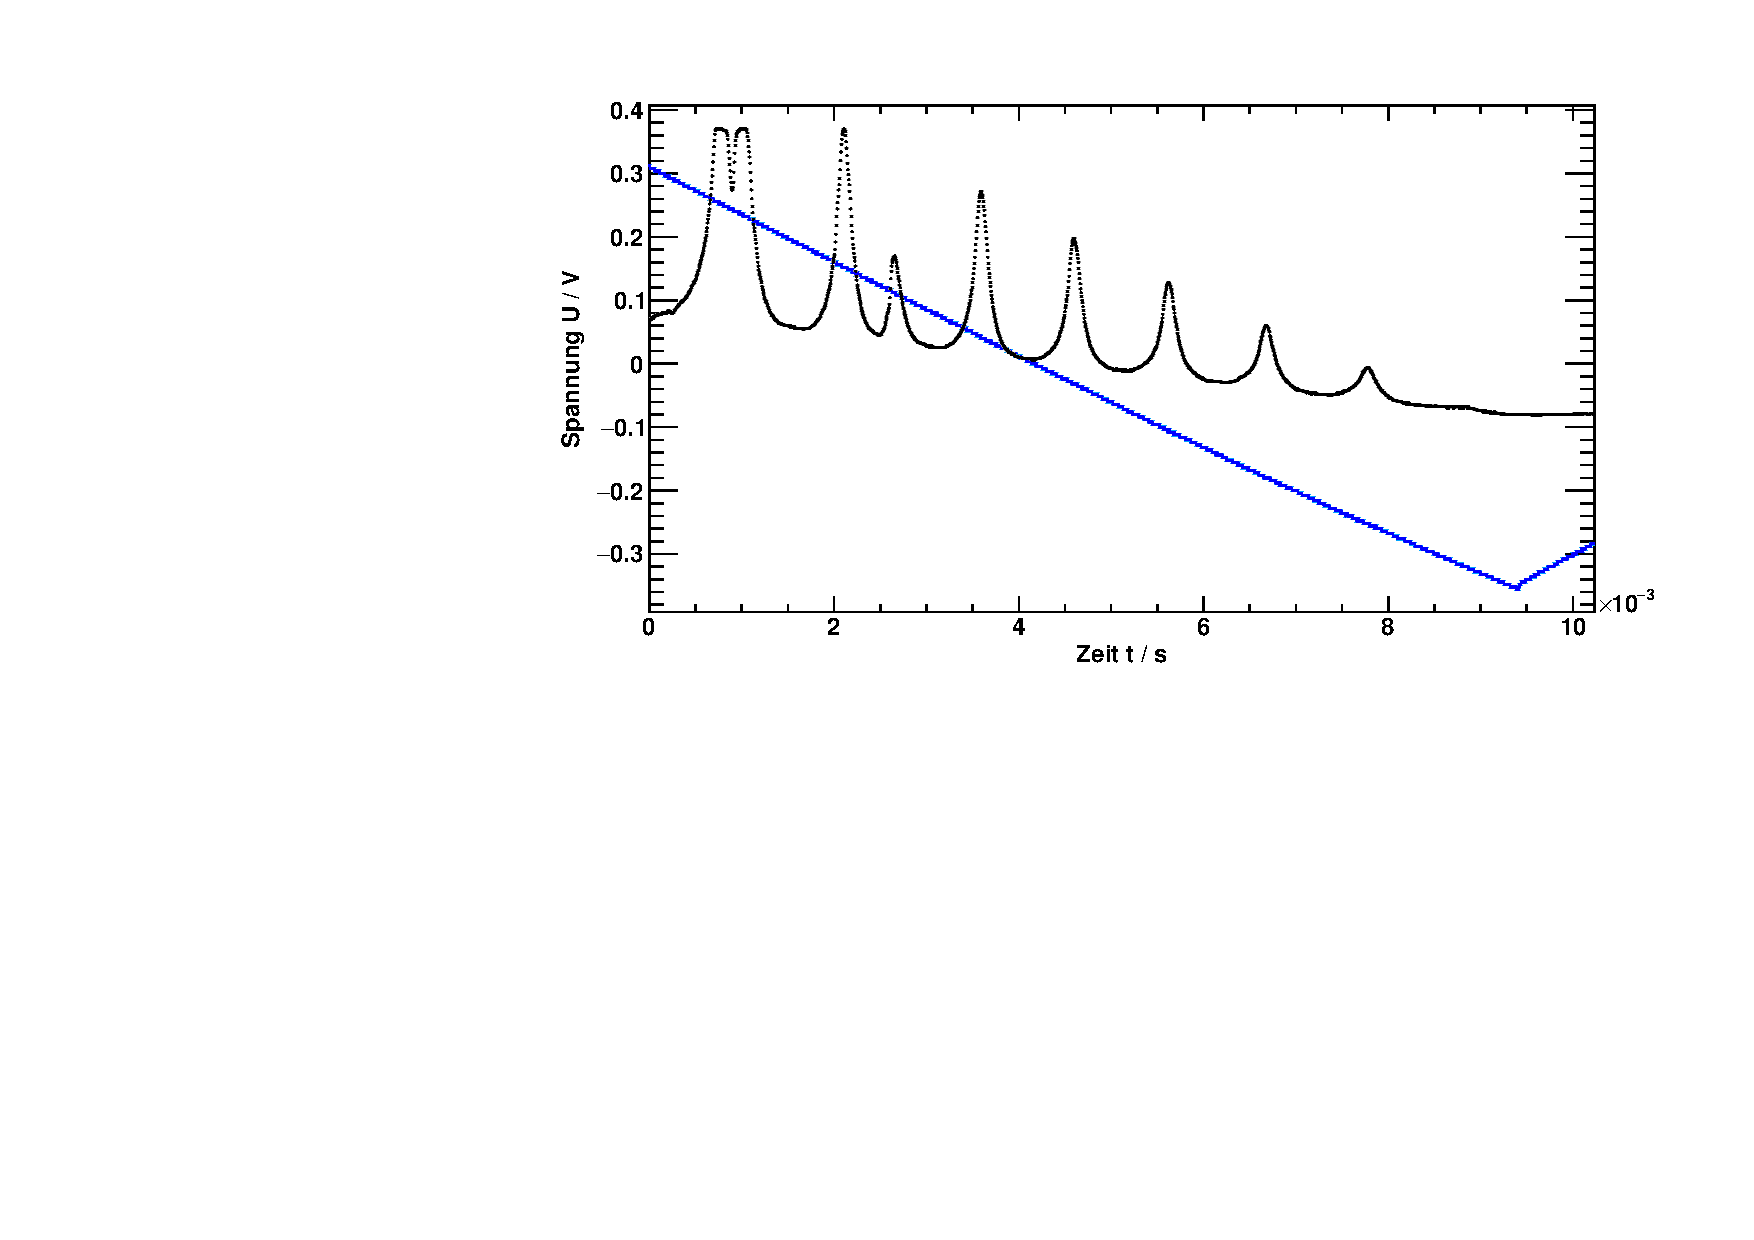
\includegraphics[width=\textwidth]{../img/down-etalon_zoom.pdf} % TODO Achsenbeschriftung
    \caption{Peaks des Etalonspektrums auf fallender Flanke.}
\end{figure}
\end{frame}


\begin{frame}
\frametitle{Auswertung: Bestimmung der Scanrate des Lasers}
\begin{figure}
    \centering
    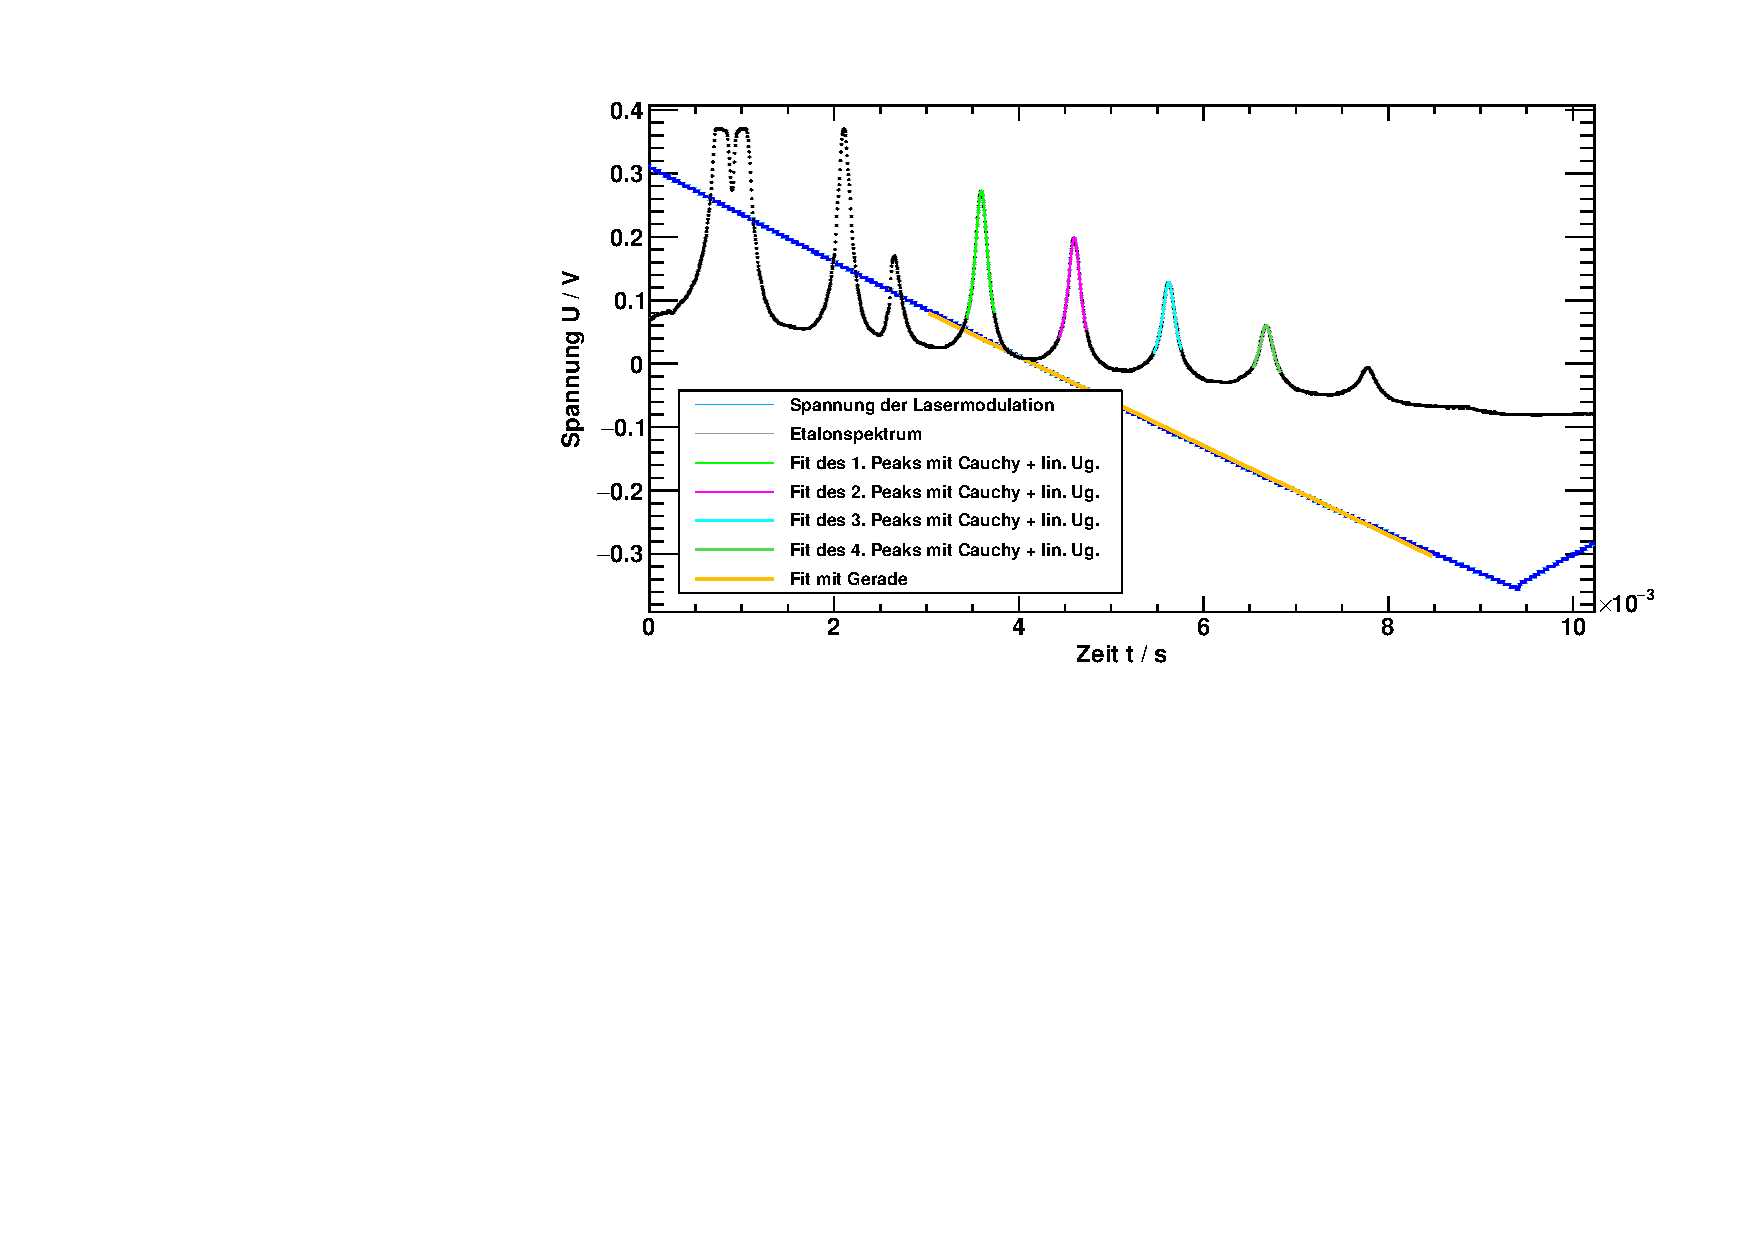
\includegraphics[width=\textwidth]{../img/down-etalon_zoom_fit.pdf}
    \caption{Fit mit Breit-Wigner-Kurven.}
\end{figure}
\end{frame}

\begin{frame}
\frametitle{Auswertung: Bestimmung der Scanrate des Lasers}
  \begin{figure}[H]
      \centering
      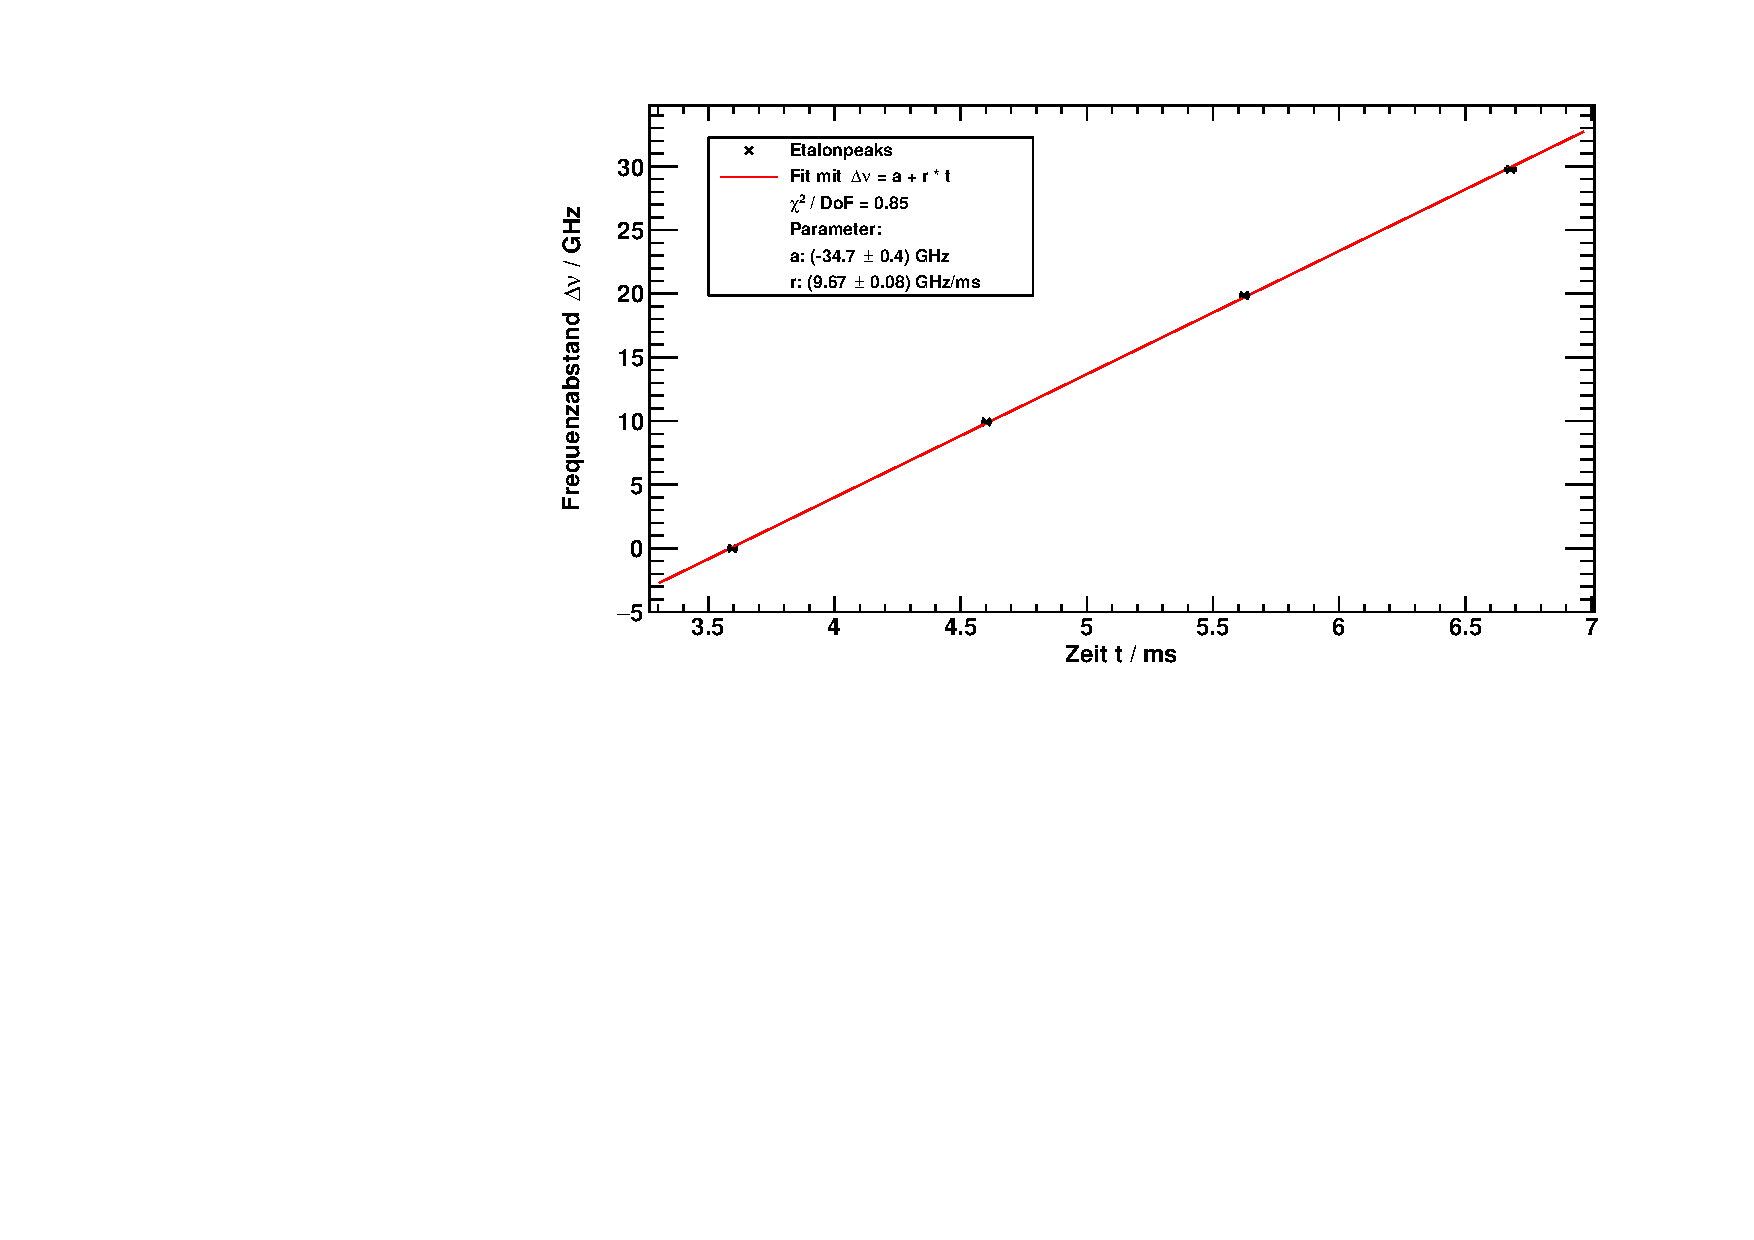
\includegraphics[width=\textwidth]{../img/down-etalon_zoom-etalon_calibration.pdf}
      \caption{Frequenzdifferenz der Etalonpeaks und ihre Positionen.}
  \end{figure}
\end{frame}


\begin{frame}
\frametitle{Auswertung: Bestimmung der Scanrate des Lasers}
Fit mit
\begin{equation*}
    \Delta \nu(t) = a + r \cdot t
\end{equation*}
\pause
Scanrate $r$ des Lasers
\begin{equation*}
    r = (9.47 \pm 0.08)\,\frac{\text{GHz}}{\text{ms}}
\end{equation*}
\end{frame}

\subsection{Hyperfeinstruktur}

\begin{frame}
\frametitle{Aufbau: Hyperfeinstrukturspektrum}
\setbeamerfont{myfont}{size*=80}
\usebeamerfont{myfont}
\begin{figure}
    \centering
    \def\svgwidth{\textwidth}
    \input{../img/aufbauHFSSpektrum.pdf_tex}
    \caption{Aufbau zur Messung des Hyperfeinstrukturspektrums.}
\end{figure}
\usebeamerfont{standard}
\begin{itemize}
  \item \textbf{Rubidiumzelle:} Füllung mit \rb{85} und \rb{87} (T$_\text{m}=39^\circ$C)
  und Puffergas Krypton ($p=1.5$\,mbar)
\end{itemize}
\end{frame}


\begin{frame}
\frametitle{Aufbau: Strahlengang}
\begin{figure}[H]
    \centering
    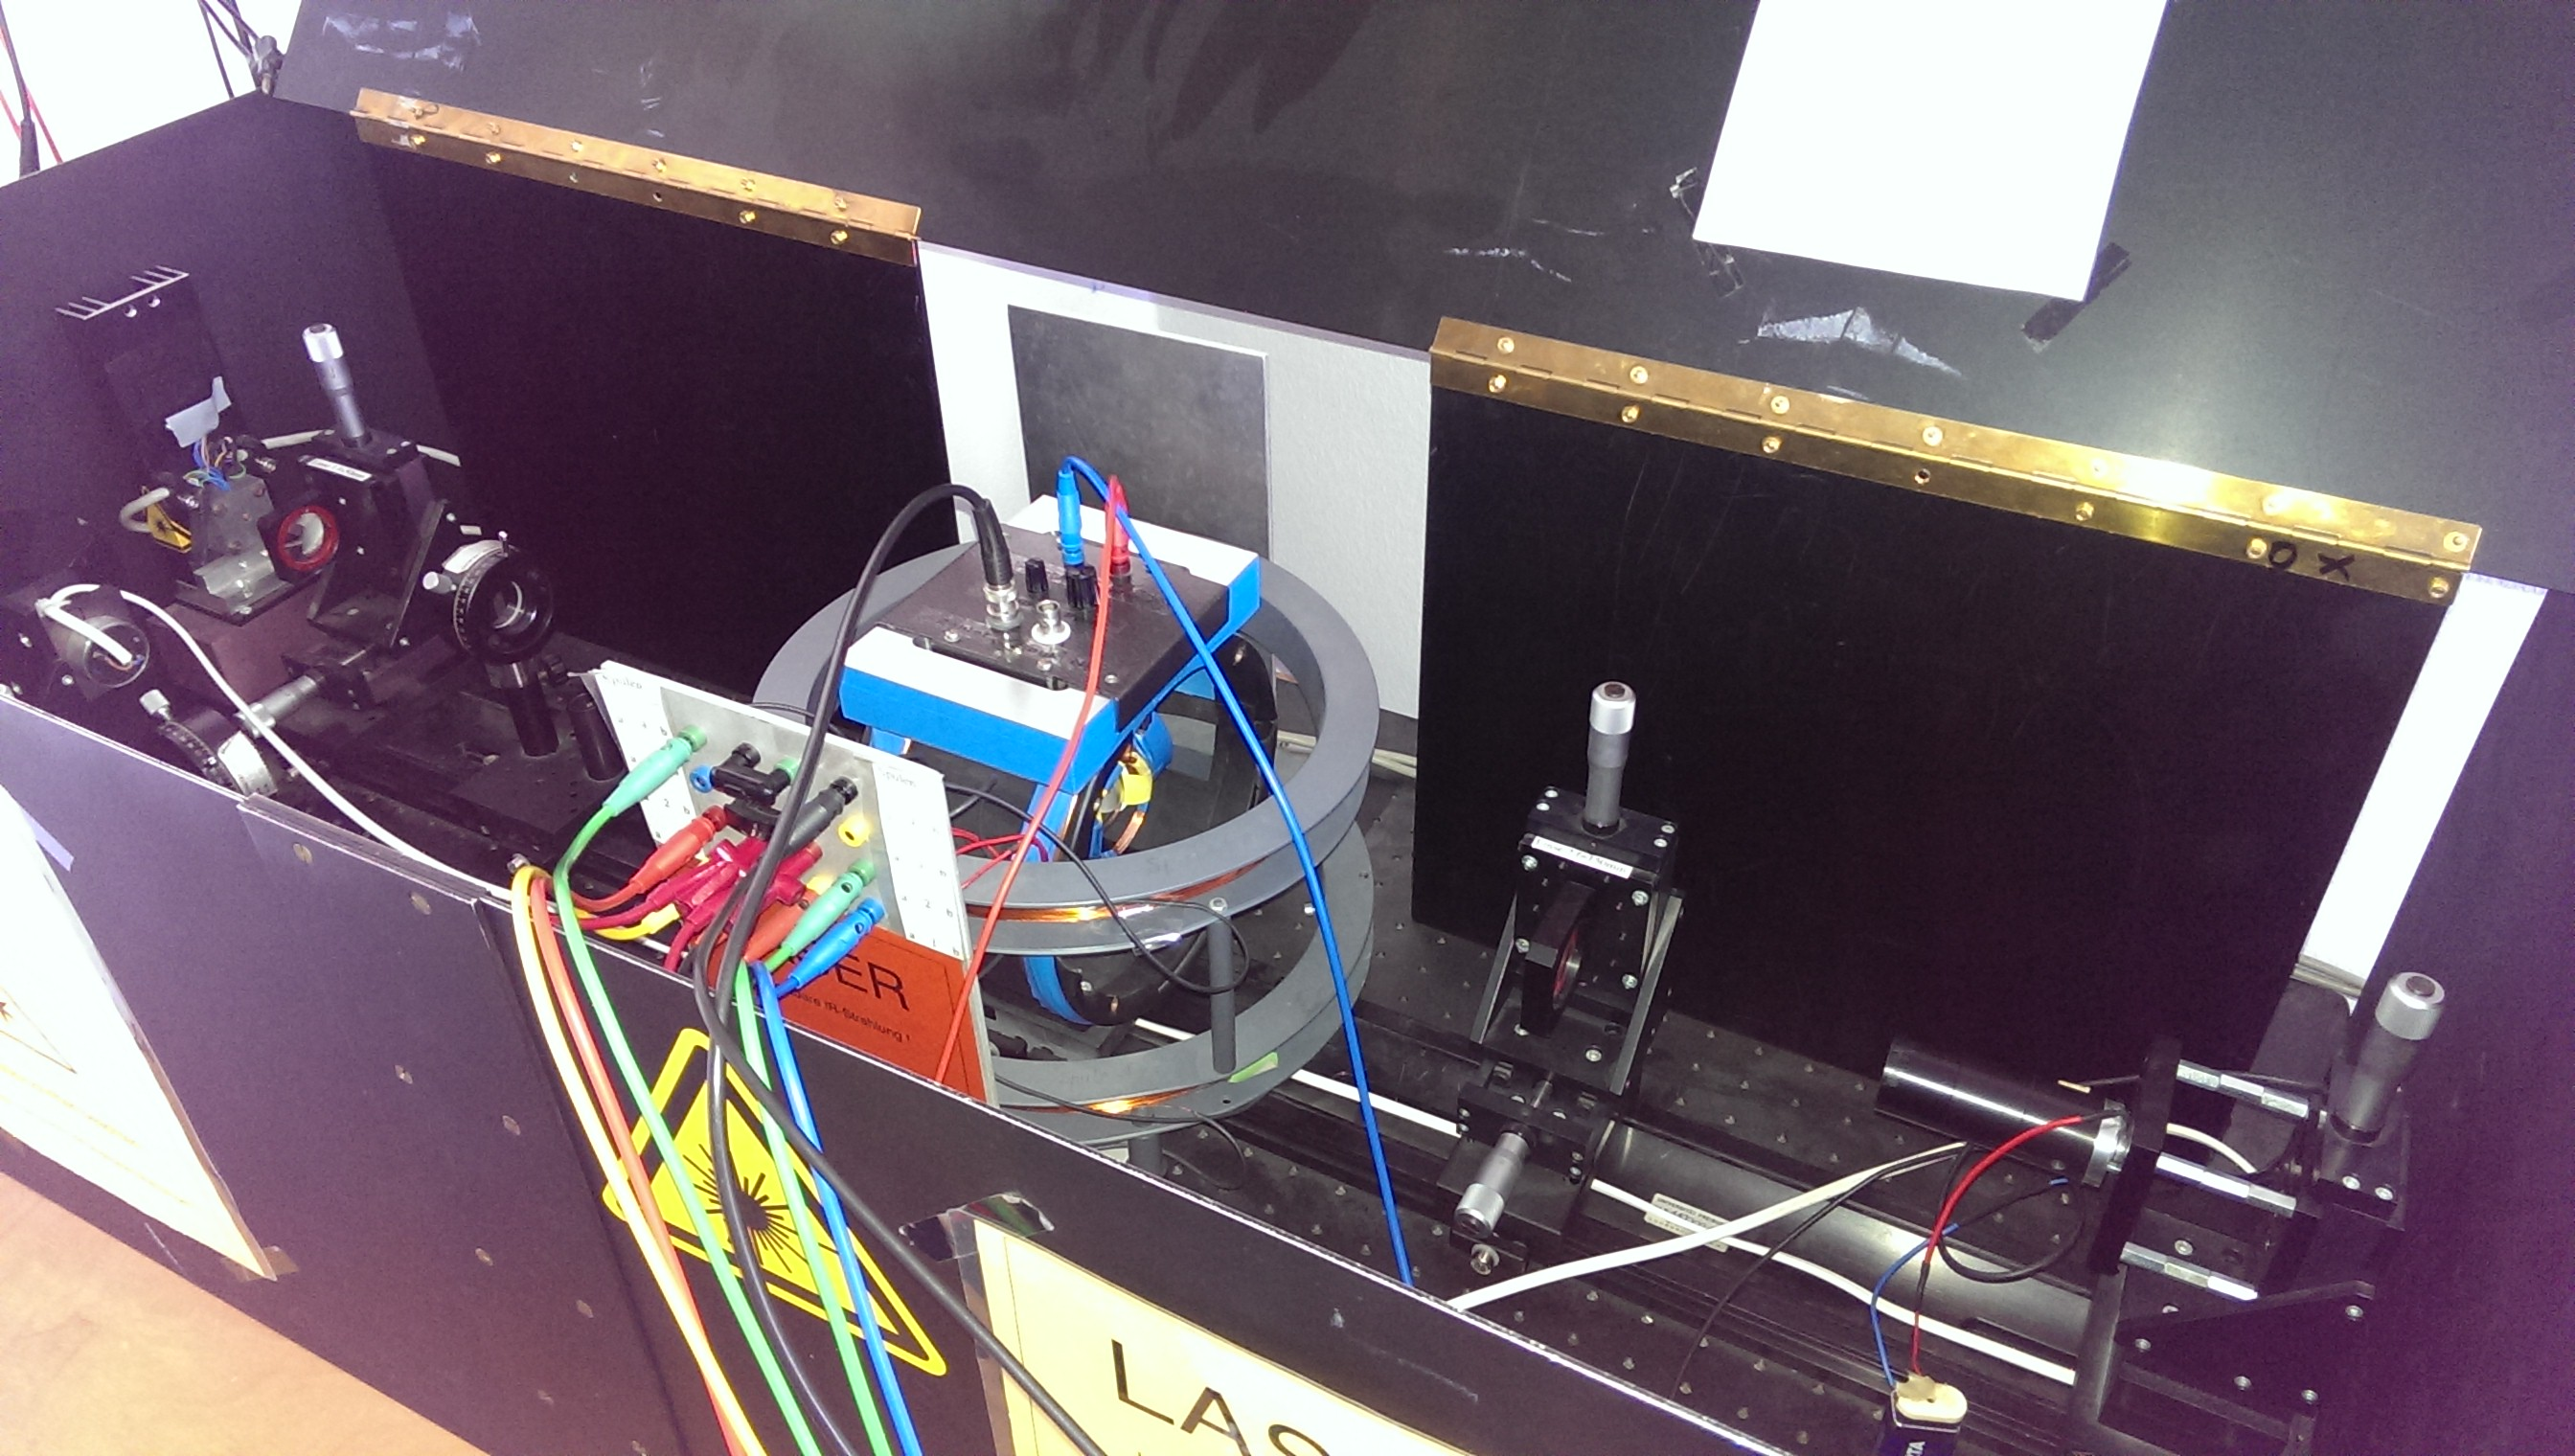
\includegraphics[width=\textwidth]{../img/aufbau_strahlengang.jpg}
    \caption{Strahlengang.}
\end{figure}
\end{frame}

\begin{frame}
\frametitle{Aufbau: Rubidiumzelle}
\begin{figure}[H]
    \centering
    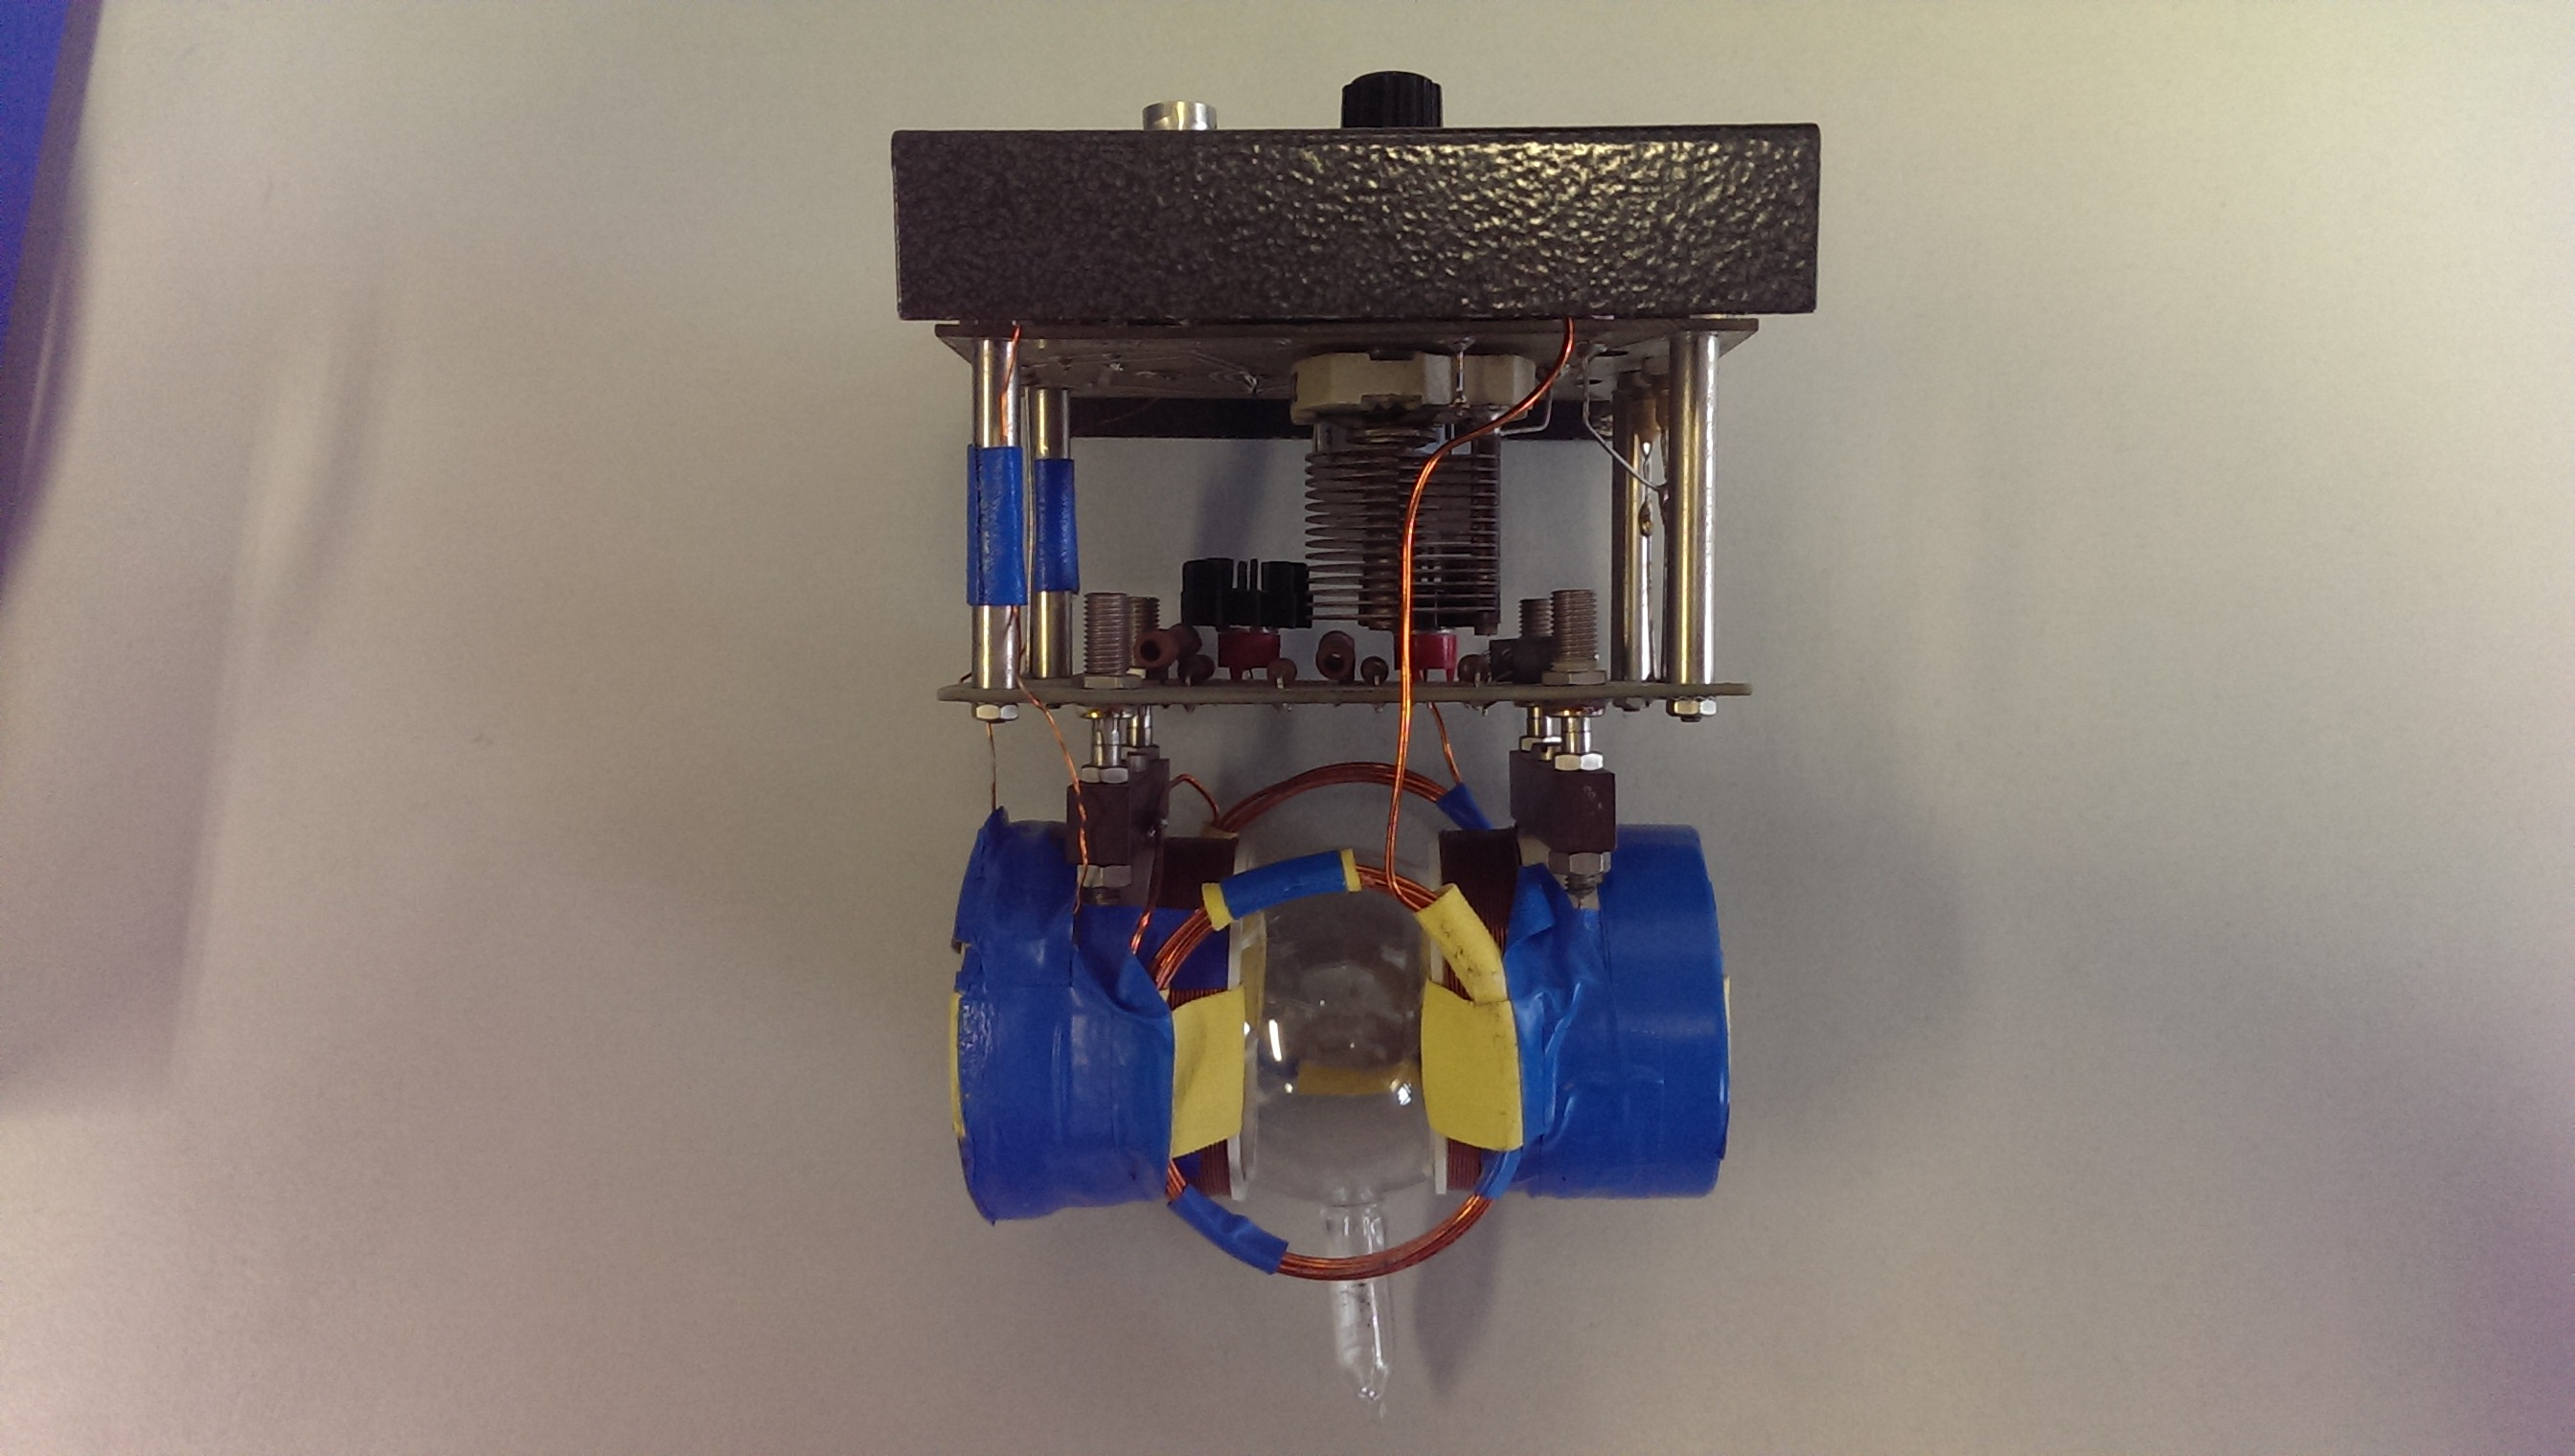
\includegraphics[width=\textwidth]{../img/aufbau_rubidiumzelle.jpg}
    \caption{Rubidiumzelle.}
\end{figure}
\end{frame}

\begin{frame}
\frametitle{Auswertung: Hyperfeinstruktur-Übergänge}
\begin{figure}[H]
    \centering
    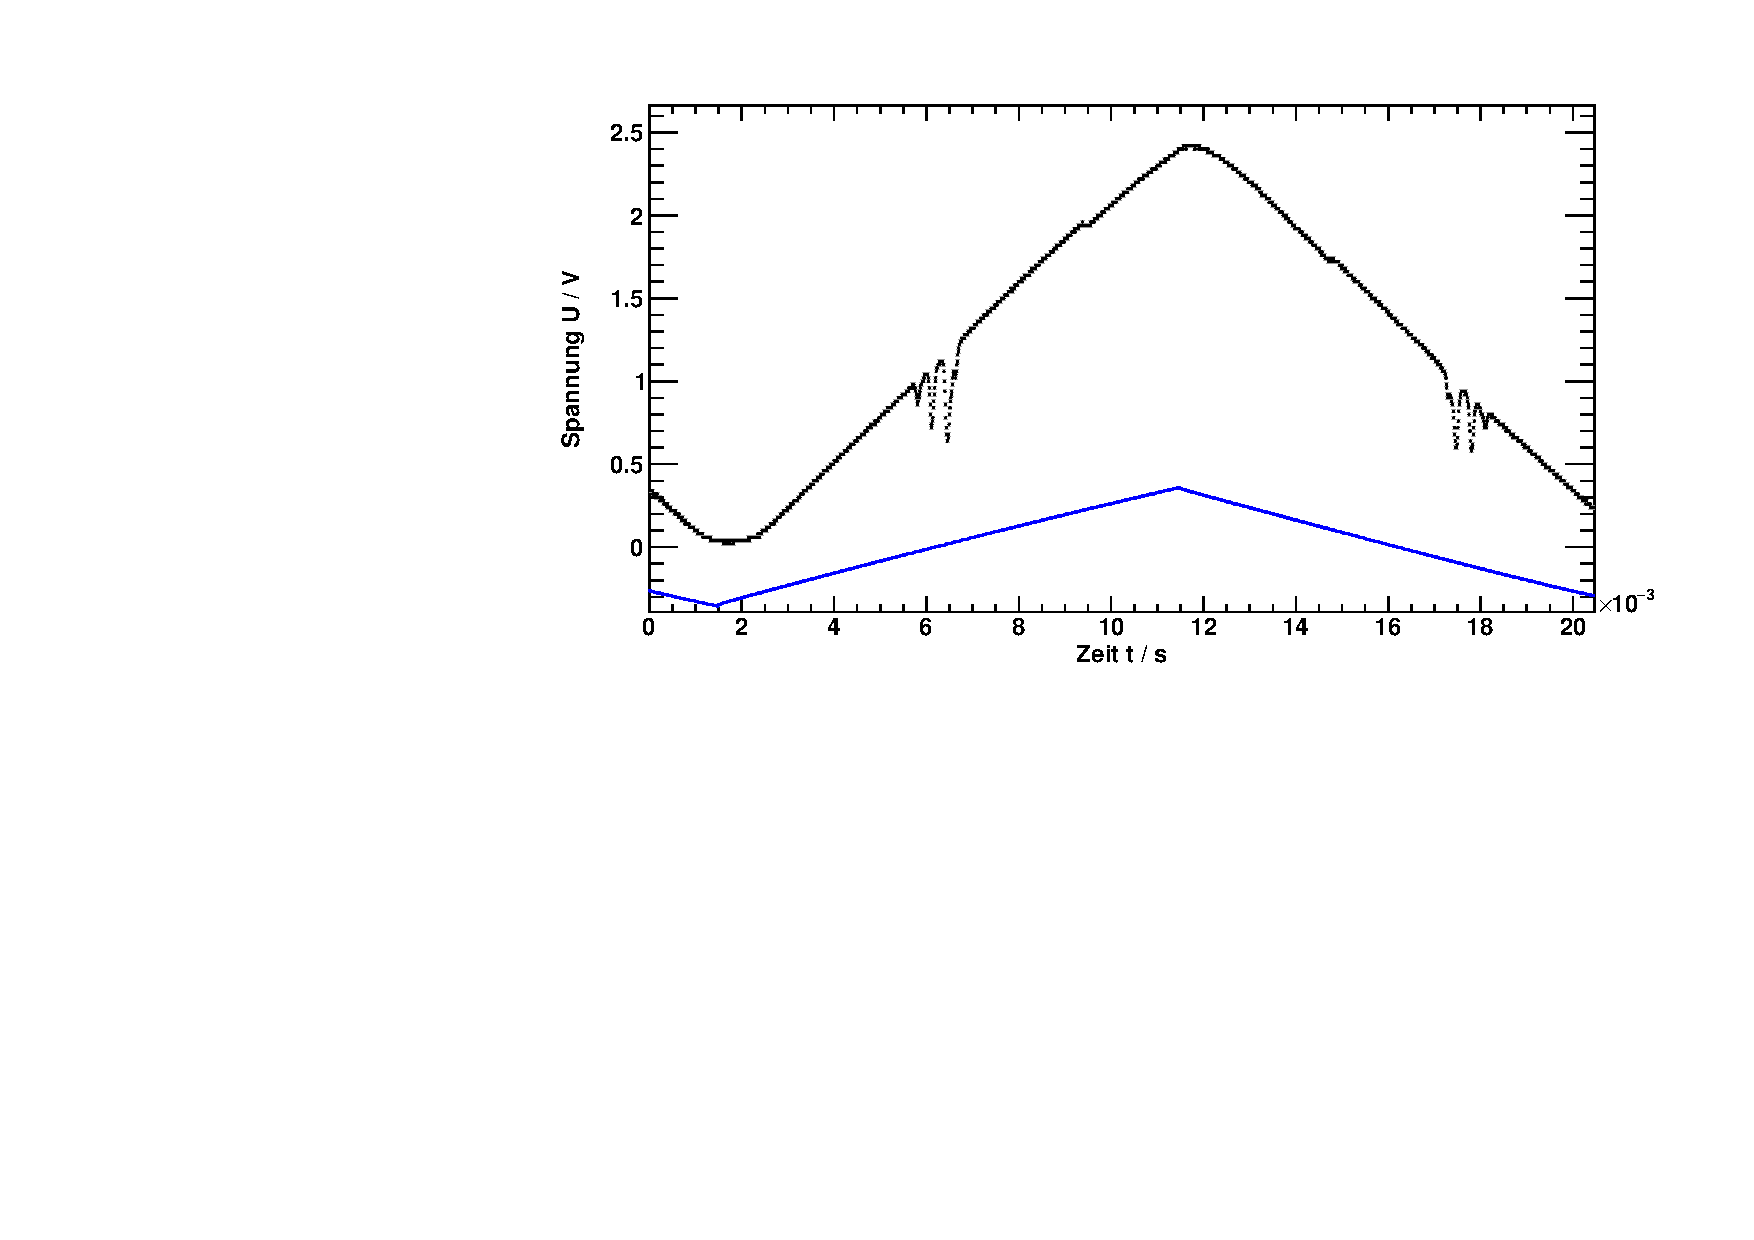
\includegraphics[width=\textwidth]{../img/down-hfs.pdf}
    \caption{Hyperfeinstrukturspektrum von Rubidium.}
\end{figure}
\end{frame}


\begin{frame}
\frametitle{Auswertung: Hyperfeinstruktur-Übergänge}
\begin{figure}[H]
    \centering
    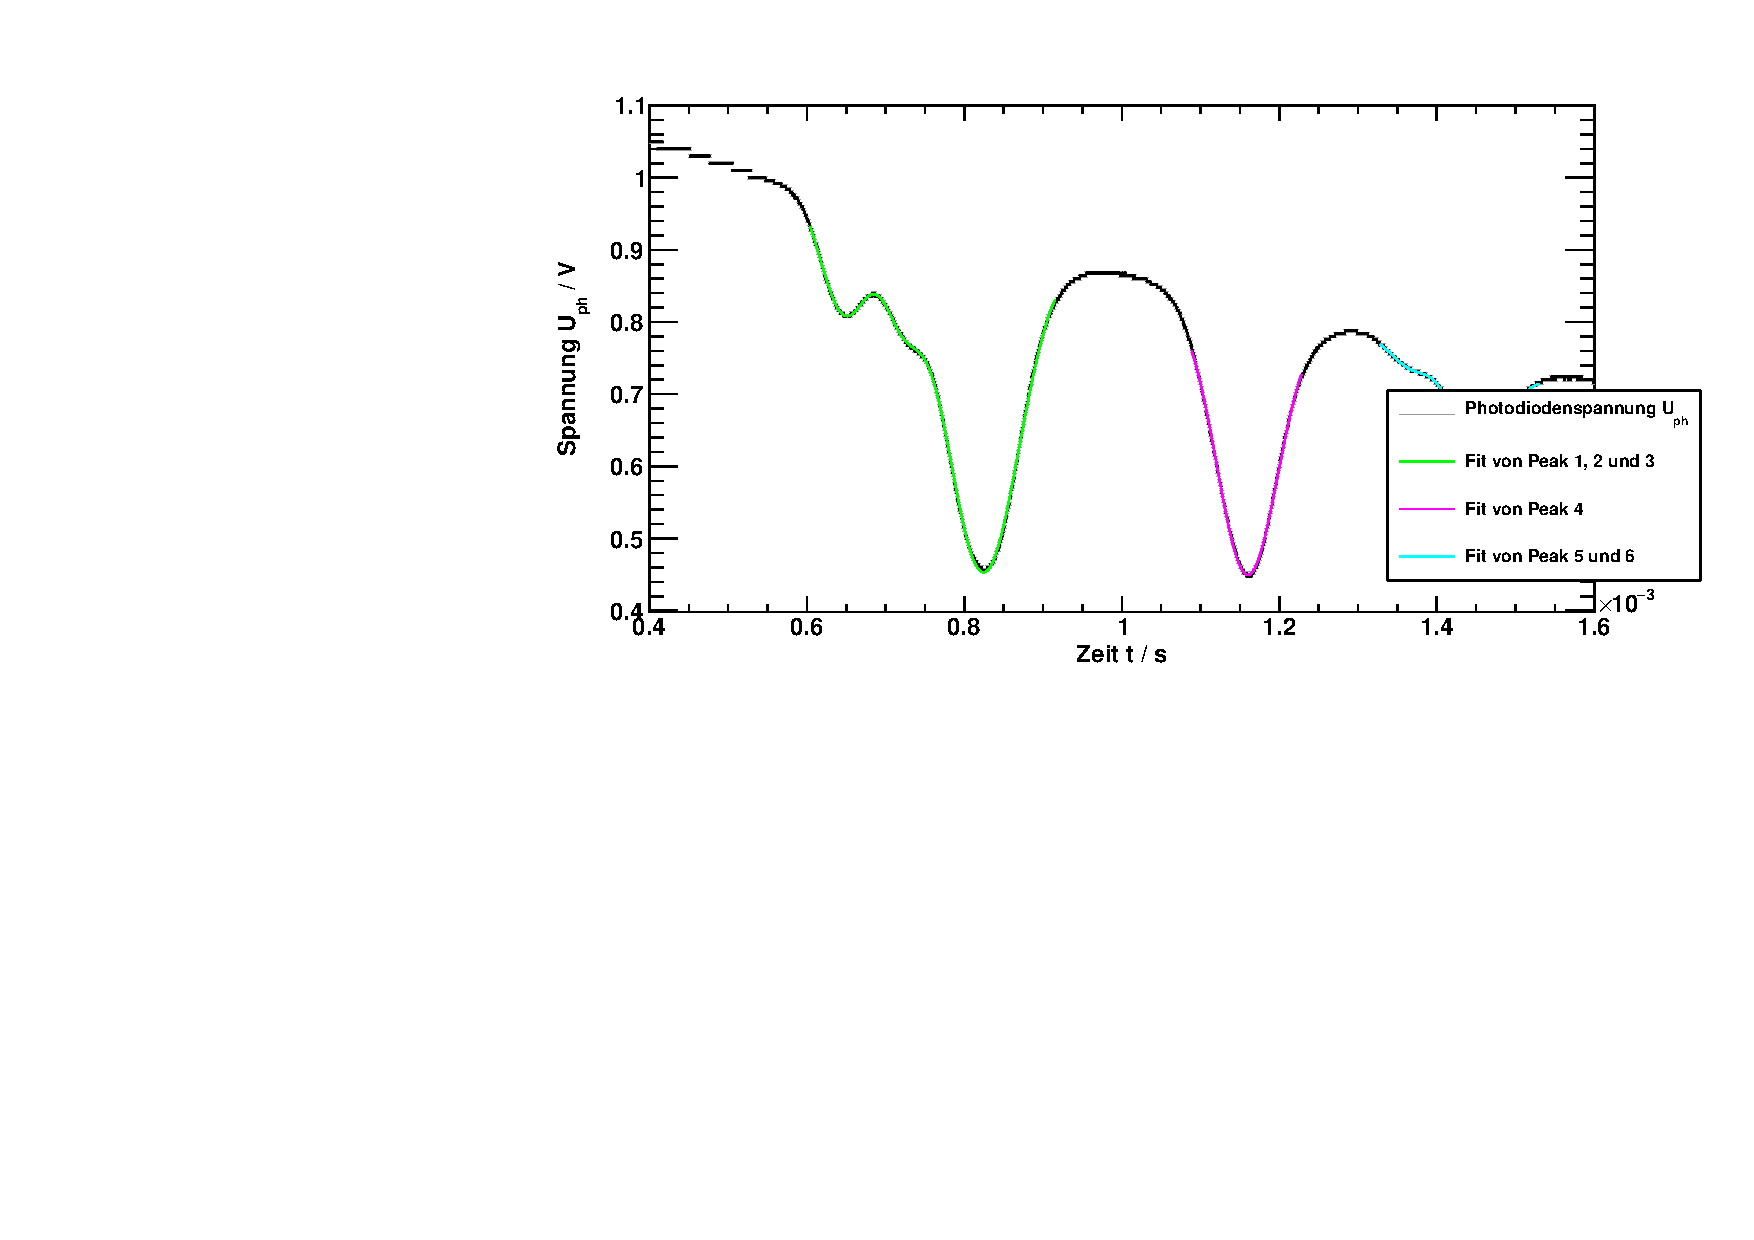
\includegraphics[width=\textwidth]{../img/down-hfs_zoom_fit.pdf}  % TODO Legend
    \caption{Fit mit überlagerten Gauß-Kurven.}
\end{figure}
\end{frame}


\begin{frame}
\frametitle{Auswertung: Berechnung der Frequenzdifferenz}
\begin{itemize}[<+->]
    \item Festlegung eines Referenzpeaks (Peak 3)
    \item Berechnung mit
    \begin{equation*}
        \Delta \nu_i = r \cdot \left( \mu_i - \mu_3 \right)
    \end{equation*}
\end{itemize}
\end{frame}


\begin{frame}
\frametitle{Auswertung: Vergleich mit theoretischen Werten}
\begin{figure}
\begin{center}
    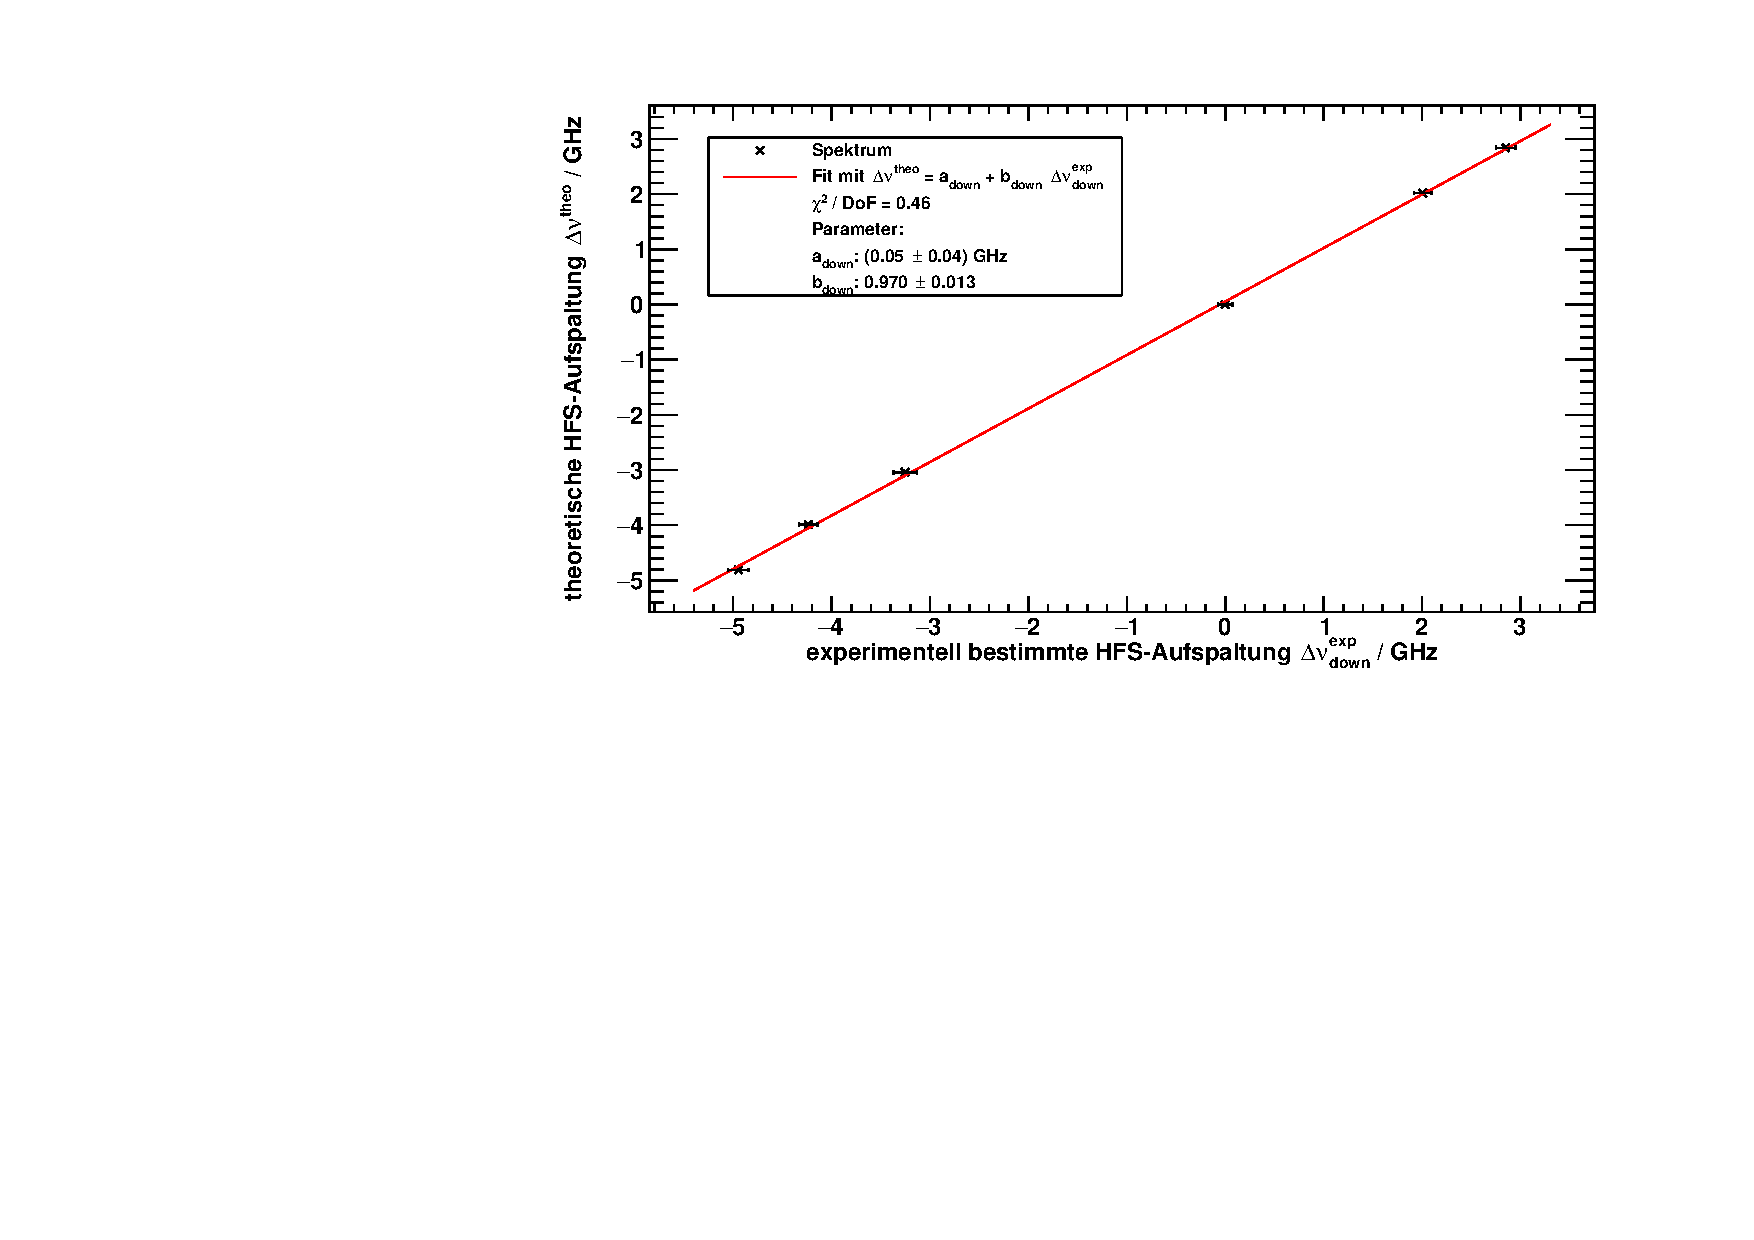
\includegraphics[width=\textwidth]{../img/down-spectrum.pdf}
    \caption{Vergleich des auf der fallenden Flanke gemessenen Hyperfeinstrukturspektrums mit den theoretischen Werten.}
\end{center}
\end{figure}
\end{frame}


\begin{frame}
\frametitle{Auswertung: Vergleich mit theoretischen Werten}
\begin{itemize}[<+->]
    \item Fit mit
    \begin{equation*}
        \Delta \nu^\text{theo} = a + b \cdot \Delta \nu^\text{exp}
    \end{equation*}
    \item Ergebnis
    \begin{equation*}
        \begin{array}{ll}
            a_\text{up} = (-0.01 \pm 0.04)\,\text{GHz} & a_\text{down} = (0.05 \pm 0.04)\,\text{GHz} \\
            b_\text{up} = 0.973 \pm 0.013 & b_\text{down} = 0.970 \pm 0.013
        \end{array}
    \end{equation*}
    \item Möglicher Fehler: Etalon im Strahlengang verkippt
    \begin{itemize}[<+->]
        \item[$\Rightarrow$] Verkleinerung des freien Spektralbereichs
        \item[$\Rightarrow$] Vergrößerung der Abstände der Peaks
        \item[$\Rightarrow$] kleinere Steigung der Vergleichsgeraden
    \end{itemize}
\end{itemize}
\end{frame}

\subsection{Intervallkonstante A}

\begin{frame}
\frametitle{Auswertung: Berechnung der Intervallkonstanten $A$}
\setbeamerfont{myfont}{size*=80}
\usebeamerfont{myfont}
\begin{figure}
    \centering
    \def\svgwidth{\textwidth}
    \input{../img/termschemahyperfein.pdf_tex}
    \caption{Hyperfeinstrukturaufspaltung der D$_1$-Linie von 
    \rb{85} und \rb{87} mit Übergängen von S$_{1/2}$ nach P$_{1/2}.$}
\end{figure}
\end{frame}


\begin{frame}
\frametitle{Auswertung: Berechnung der Intervallkonstanten $A$}
\setbeamerfont{myfont}{size*=80}
\usebeamerfont{myfont}
\begin{figure}
    \centering
    \def\svgwidth{\textwidth}
    \input{../img/termschemahyperfein_linien.pdf_tex}
    \caption{Hyperfeinstrukturaufspaltung der D$_1$-Linie von 
    \rb{85} und \rb{87} mit Übergängen von S$_{1/2}$ nach P$_{1/2}.$}
\end{figure}
\end{frame}


\begin{frame}
\frametitle{Auswertung: Berechnung der Intervallkonstanten $A$}
\setbeamerfont{myfont}{size*=80}
\usebeamerfont{myfont}

\begin{figure}
    \centering
    \def\svgwidth{\textwidth}
    \input{../img/HFSspect_theo.pdf_tex}
    \caption{Spektrallinien der Hyperfeinstruktur des ${}^2\text{S}_{1/2}$\,-\,${}^2\text{P}_{1/2}$\,-\,Übergangs
    von \rb{85} und \rb{87}.}
\end{figure}

\end{frame}


\begin{frame}
\frametitle{Auswertung: Berechnung der Intervallkonstanten $A$}
\begin{equation*}
    \begin{split}
        \Delta E &= \Delta \nu \cdot h = A (F + 1) \\
        \Rightarrow A &= \frac{\Delta \nu \cdot h}{F + 1}
    \end{split}
\end{equation*}
\begin{table}
\caption{Errechnete HFS-Intervallkonstanten $A$ für das ${}^2\text{S}_{1/2}$ Niveau von \rb{85} und für das ${}^2\text{S}_{1/2}$- und ${}^2\text{P}_{1/2}$ Niveau von \rb{87}.}
\begin{center}
\begin{tabular}{|c|c|c|c|}
  \hline
  Isotop / Feinstruktur & $A^\text{Lit.}$ / \textmu eV & $A^\text{exp}$ / \textmu eV \\ \hline
  \rb{85}: ${}^2\text{S}_{1/2}$ & 4.185 & $4.47 \pm 0.14$ \\ \hline
  \rb{87}: ${}^2\text{S}_{1/2}$ & 14.13 & $14.49 \pm 0.14$ \\ \hline
  \rb{87}: ${}^2\text{P}_{1/2}$ & 1.692 & $1.61 \pm 0.14$ \\ \hline
\end{tabular}
\end{center}
\label{tab:hfs:intervalconsts}
\end{table}
\end{frame}